\chapter{Arhitektura i dizajn sustava}
		
	
	Arhitektura se može podijeliti na tri podsustava:
	\begin{enumerate}
		\item Web poslužitelj
		\item Web aplikacija
		\item Baza podataka
	\end{enumerate}
	
	\underline{Web preglednik} je program koji korisniku omogućuje pregled web-stranica i multimedijalnih sadržaja vezanih uz njih. Svaki internetski preglednik je prevoditelj. Dakle, stranica je pisana u kodu koji preglednik nakon toga interpretira kao nešto svakome razumljivo. Korisnik putem web preglednika šalje zahtjev web poslužitelju.
	
	\underline{Web poslužitelj} osnova je rada web aplikacije. Njegova primarna zadaća je komunikacija klijenta s aplikacijom. Komunikacija s odvija preko HTTPS protokola (engl. \textit{Hyper Text Transfer Protocol Secure}) protokola, koji je protokol u prijenosu informacija na webu. Poslužitelj je onaj koji pokreće web aplikaciju te joj prosljeđuje zahtjev.
	
	Korisnik koristi \underline{web aplikaciju} za obrađivanje željenih zahtjeva. Web aplikacija obrađuje zahtjev te ovisno o zahtjevu pristupa bazi podataka nakon čega preko poslužitelja vraća korisniku odgovor u obliku HTML dokumenta vidljivog u web pregledniku. Programski jezik kojeg smo odabrali za izradu naše web aplikacije je JavaScript te Express radni okvir. Odabrana razvojna okolina je Visual Studio Code. Express podržava MVC koncept i time olakšava razvoj web aplikacije. Arhitektura same aplikacije je podijeljena ne klijentski i poslužiteljski dio. Klijentski dio je izgrađen pomoću HTML-a i JavaScripta. Klijentski dio korisnici koriste za interakciju s aplikacijom kroz web preglednik. Klijentski dio šalje zahtjeve poslužitelju ovisno o akcijama korisnika. Poslužiteljski dio izgrađen je pomoću Express razvojnog okvira te primjenjuje MVC koncept. Karakteristika takvog pristupa je razdvajanje domena problema koja rezultira učinkovitijom podjelom članova po timovima. MVC također doprinosi i modularnosti koda i njegovoj čitljivosti.

	
		

		

				
		\section{Baza podataka}

		
		Za potrebu našeg sustava koristiti ćemo relacijsku bazu podataka koja svojom strukturom olakšava modeliranje interakcije u sustavu. Osnovna gradivna jedinica baze je relacija, to jest imenovana tablica s definiranim atributima. Zadaća baze podataka je brza, jednostavna i robusna pohrana, alteracija i dohvat podataka za daljnju obradu. Baza podataka ove aplikacije sastoji se od sljedećih entiteta:
		
		\begin{itemize}
			\item Korisnik
			\item Ima izgled
			\item Tenk
			\item Igrao je
			\item Igra
			\item Mapa

		\end{itemize}
		
			\subsection{Opis tablica}
				
			\textbf{Korisnik} Ovaj entitet sadrži sve bitne podatke o korisniku. Sadrži atribute: korisničko ime, lozinka, email, razinu ovlasti te datum rođenja. Ovaj entitet je u vezi \textit{One-to-many} s entitetom Igrao je preko korisničkog imena te u vezi \textit{One-to-many} s entitetom Ima izgled preko korisničkog imena.
				
				\begin{longtabu} to \textwidth {|X[6, l]|X[6, l]|X[20, l]|}
					
					\hline \multicolumn{3}{|c|}{\textbf{Korisnik}}	 \\[3pt] \hline
					\endfirsthead
					
					\hline \multicolumn{3}{|c|}{\textbf{Korisnik}}	 \\[3pt] \hline
					\endhead
					
					\hline 
					\endlastfoot
					
					\cellcolor{LightGreen}korisničko ime & VARCHAR	&  	jedinstveni identifikator korisnika 	\\ \hline
					lozinka	& VARCHAR & hash lozinke  	\\ \hline 
					email & VARCHAR & e-mail adresa korisnika  \\ \hline 
					razina ovlasti & INT	& razina ovlasti korisnika\\ \hline 
					
					
				\end{longtabu}
			
			\textbf{Ima izgled} Ovaj entitet je spojni entitet entiteta Korisnik i Tenk. Sadrži atribute: korisničko ime i tenkId. Ovaj entitet je u vezi \textit{Many-to-one} s entitetom Korisnik preko korisničkog imena te u vezi \textit{Many-to-one} s entitetom Tenk preko tenkId-a.
				
				\begin{longtabu} to \textwidth {|X[6, l]|X[6, l]|X[20, l]|}
					
					\hline \multicolumn{3}{|c|}{\textbf{Ima izgled}}	 \\[3pt] \hline
					\endfirsthead
					
					\hline \multicolumn{3}{|c|}{\textbf{Ima izgled}}	 \\[3pt] \hline
					\endhead
					
					\hline 
					\endlastfoot
					
					\cellcolor{LightGreen}korisničko ime & VARCHAR	&  	jedinstveni identifikator korisnika 	\\ \hline
					\cellcolor{LightGreen}tenkId	& VARCHAR & jedinstveni identifikator tenka  	\\ \hline 
					
					
				\end{longtabu}
			
			
			\textbf{Tenk} Ovaj entitet sadržava informacije o tenku. Sadrži atribute: tenkId, ime tenka, razina otključavanja. Ovaj entitet je u vezi \textit{Many-to-many} s entitetom Ima izgled preko tenkId-a.
			
				\begin{longtabu} to \textwidth {|X[6, l]|X[6, l]|X[20, l]|}
					
					\hline \multicolumn{3}{|c|}{\textbf{Tenk}}	 \\[3pt] \hline
					\endfirsthead
					
					\hline \multicolumn{3}{|c|}{\textbf{Tenk}}	 \\[3pt] \hline
					\endhead
					
					\hline 
					\endlastfoot
					
					\cellcolor{LightGreen}tenkId & VARCHAR	&  	jedinstveni identifikator tenka 	\\ \hline
					ime tenka	& VARCHAR & naziv tenka  	\\ \hline 
					razina otključavanja & INT & razina na kojoj korisnik otključava ovaj tenk  \\ \hline 
					
					
				\end{longtabu}
			
			\textbf{Igrao je} Ovaj entitet je spojni entitet entiteta Korisnik i Igra. Sadrži atribute: korisničko ime, broj bodova, puta uništio, puta uništen te igraId. Ovaj entitet je u vezi \textit{Many-to-one} s entitetom Korisnik preko korisničkog imena te u vezi \textit{One-to-many} s entitetom Igra preko igraId.
			
				\begin{longtabu} to \textwidth {|X[6, l]|X[6, l]|X[20, l]|}
					
					\hline \multicolumn{3}{|c|}{\textbf{Igrao je}}	 \\[3pt] \hline
					\endfirsthead
					
					\hline \multicolumn{3}{|c|}{\textbf{Igrao je}}	 \\[3pt] \hline
					\endhead
					
					\hline 
					\endlastfoot
					
					\cellcolor{LightGreen}korisničko ime & VARCHAR	&  	jedinstveni identifikator korisnika 	\\ \hline
					\cellcolor{LightGreen}igraId	& INT & jedinstveni idenitifikator igre  	\\ \hline 
					puta uništio & INT & broj neprijatelja koje je korisnik uništio za vrijeme igre  \\ \hline
					puta uništen & INT & broj puta koje je korisnik bio uništen za vrijeme igre  \\ \hline
					
					
				\end{longtabu}
			
			\textbf{Igra} Ovaj entitet sadrži informacije o odigranoj igri. Sadrži atribute: igraId, vrijeme početka, vrijeme kraja, mapaId. Ovaj entitet je u vezi \textit{One-to-many} s entitetom Igrao je preko igraId-a te u vezi \textit{Many-to-one} s entitetom Mapa.
			
				\begin{longtabu} to \textwidth {|X[6, l]|X[6, l]|X[20, l]|}
					
					\hline \multicolumn{3}{|c|}{\textbf{Igra}}	 \\[3pt] \hline
					\endfirsthead
					
					\hline \multicolumn{3}{|c|}{\textbf{Igra}}	 \\[3pt] \hline
					\endhead
					
					\hline 
					\endlastfoot
					
					\cellcolor{LightGreen}igraId & SERIAL INT	&  	jedinstveni identifikator igre 	\\ \hline
					\cellcolor{LightBlue}mapaId	& INT & jedinstveni identifikator mape  	\\ \hline 
					vrijeme početka & TIMESTAMP & trenutak početka igre  \\ \hline
					vrijeme kraja & TIMESTAMP & trenutak kraja igre  \\ \hline
					
					
				\end{longtabu}
			
			\textbf{Mapa} Ovaj entitet sadrži informacije o mapama. Sadrži atribute: mapaId te zahtjevnost mape. Ovaj entitet je u vezi \textit{One-to-many} s entitetom Igra preko mapaId-a.
			
				\begin{longtabu} to \textwidth {|X[6, l]|X[6, l]|X[20, l]|}
					
					\hline \multicolumn{3}{|c|}{\textbf{Mapa}}	 \\[3pt] \hline
					\endfirsthead
					
					\hline \multicolumn{3}{|c|}{\textbf{Mapa}}	 \\[3pt] \hline
					\endhead
					
					\hline 
					\endlastfoot
					
					\cellcolor{LightBlue}mapaId	& INT & jedinstveni identifikator mape  	\\ \hline 
					zahtjevnost mape & INT & zahtjevnost mape za igrati na njoj  \\ \hline
					
					
				\end{longtabu}
				
			
			\subsection{Dijagram baze podataka}
				
				\begin{figure}[h]
					\centering
					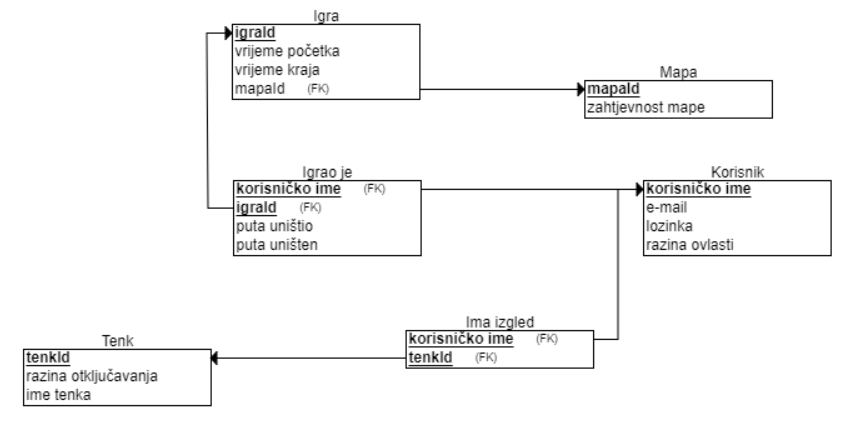
\includegraphics[width=18.5cm,height=10cm]{./databaseDiagram}
					\caption{Dijagram baze podataka}
					\label{fig:uc}
				\end{figure}
			
			\eject
			
			
		\section{Dijagram razreda}
		
		Na slici 4.2 prikazani su razredi koji pripadaju \textit{backend} dijelu MVC arhitekture. Razred Objekt je razred kojeg nasljeđuju svi objekti koji se pojavljuju na igraćem polju. Trenutno su to samo razredi Projectile i Tank. Za svaki tenk je vezana kolekcija svih projektila koje je ispalio, a da su još uvijek u igraćem polju. Također, postoji i razred Game koji reprezentira jednu igru. Budući da je moguće imati više igara u tijeku, moguće je imati i više instanci tog razreda. U jednoj igri može biti više igrača(tenkova) dok jedan igrač može trenutno biti u samo jednoj igri. U budućim iteracijama planira se više razreda objekata na mapi koji nasljeđuju razred Object. Budući da JavaScript ne razlikuje privatne, zaštićene i javne metode i atribute oni nisu ni navedeni.
			
			\begin{figure}[h]
				\centering
				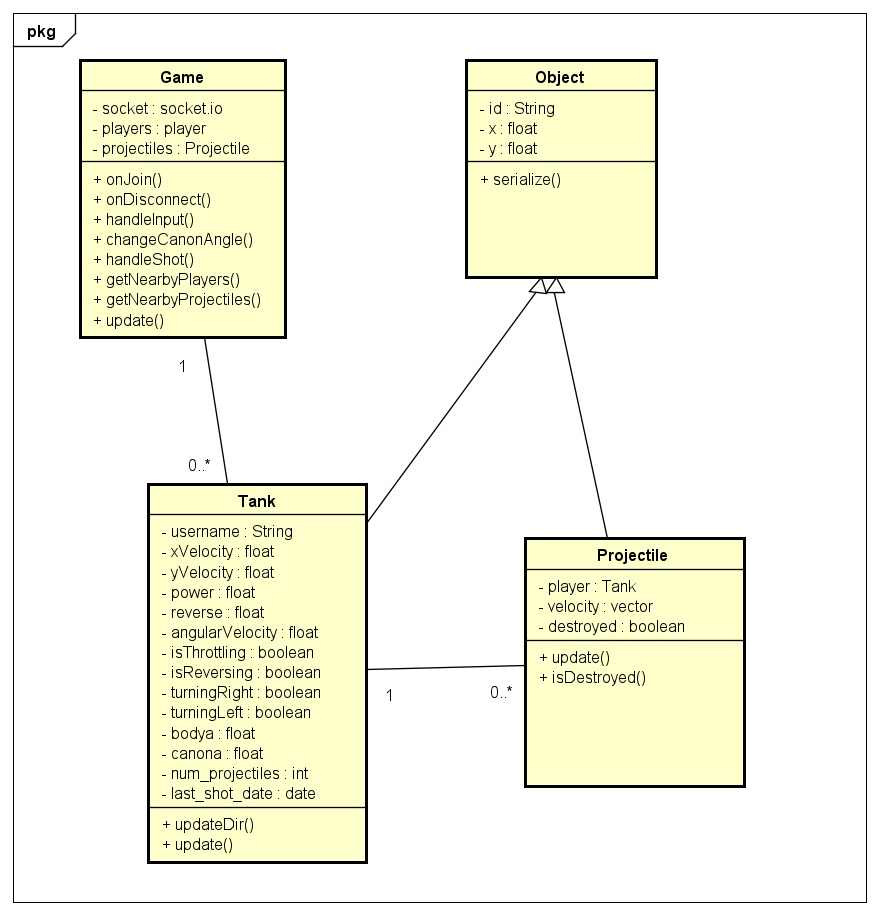
\includegraphics[width=16cm,height=12cm]{classDiagram}
				\caption{Dijagram razreda}
				\label{fig:uc}
			\end{figure}
			
			
			\newpage
			\textbf{\textit{dio 2. revizije}}\\			
			
			\textit{Prilikom druge predaje projekta dijagram razreda i opisi moraju odgovarati stvarnom stanju implementacije}
			
			
			
			\eject
		
		\section{Dijagram stanja}
			
			{UML dijagram stanja opisuje dinamičko ponašanje dijela sustava. Prikazuje stanja te prijelaze u neka druga stanja temeljene na nekim događajima. U ovom slučaju događaje određuje registrirani korisnik. Najprije, klikom na "Moj račun" korisniku se otvara izbornik s različitim mogućnostima koje može odabrati sve dok ne odluči kliknuti "Odjava". Korisnik može pregledati vlastitu statistiku ili resetirati statistiku. Kada će potvrditi resetiranje statistike, ona će se u bazi podataka postaviti na 0. Također, korisnik može pretražiti igrače. Kada odabere opciju "Pretraži igrače", automatski se pojavi polje za upis imena željenog igrača. U izborniku se nudi i promjena izgleda vozila koje je korisnik otključao. Klikom na "Promjeni podatke", korisnik može promijeniti svoje podatke tako da upiše novu zaporku i zatim spremi podatke. Korisnik može i obrisati svoj račun klikom na gumb "Obrši račun" čime će se iz baze podataka automatski korisnik obrisati. Nakon mogućih opcija koje korisnik može odabrati na "Moj račun", on također ulazi u samo igru klikom na gumb "Igraj". Nakon toga, server će tražiti rundu, ali odmah po ulasku u stanje traženja runde iz baze podataka će dobaviti podatke o iskustvu kako bi pronašao odgovarajuću rundu. Ako runda nije pronađena, postupak će se ponoviti, a u suprotnom korisnik ulazi u rundu.}
		
			
			\begin{figure}[h]
				\centering
				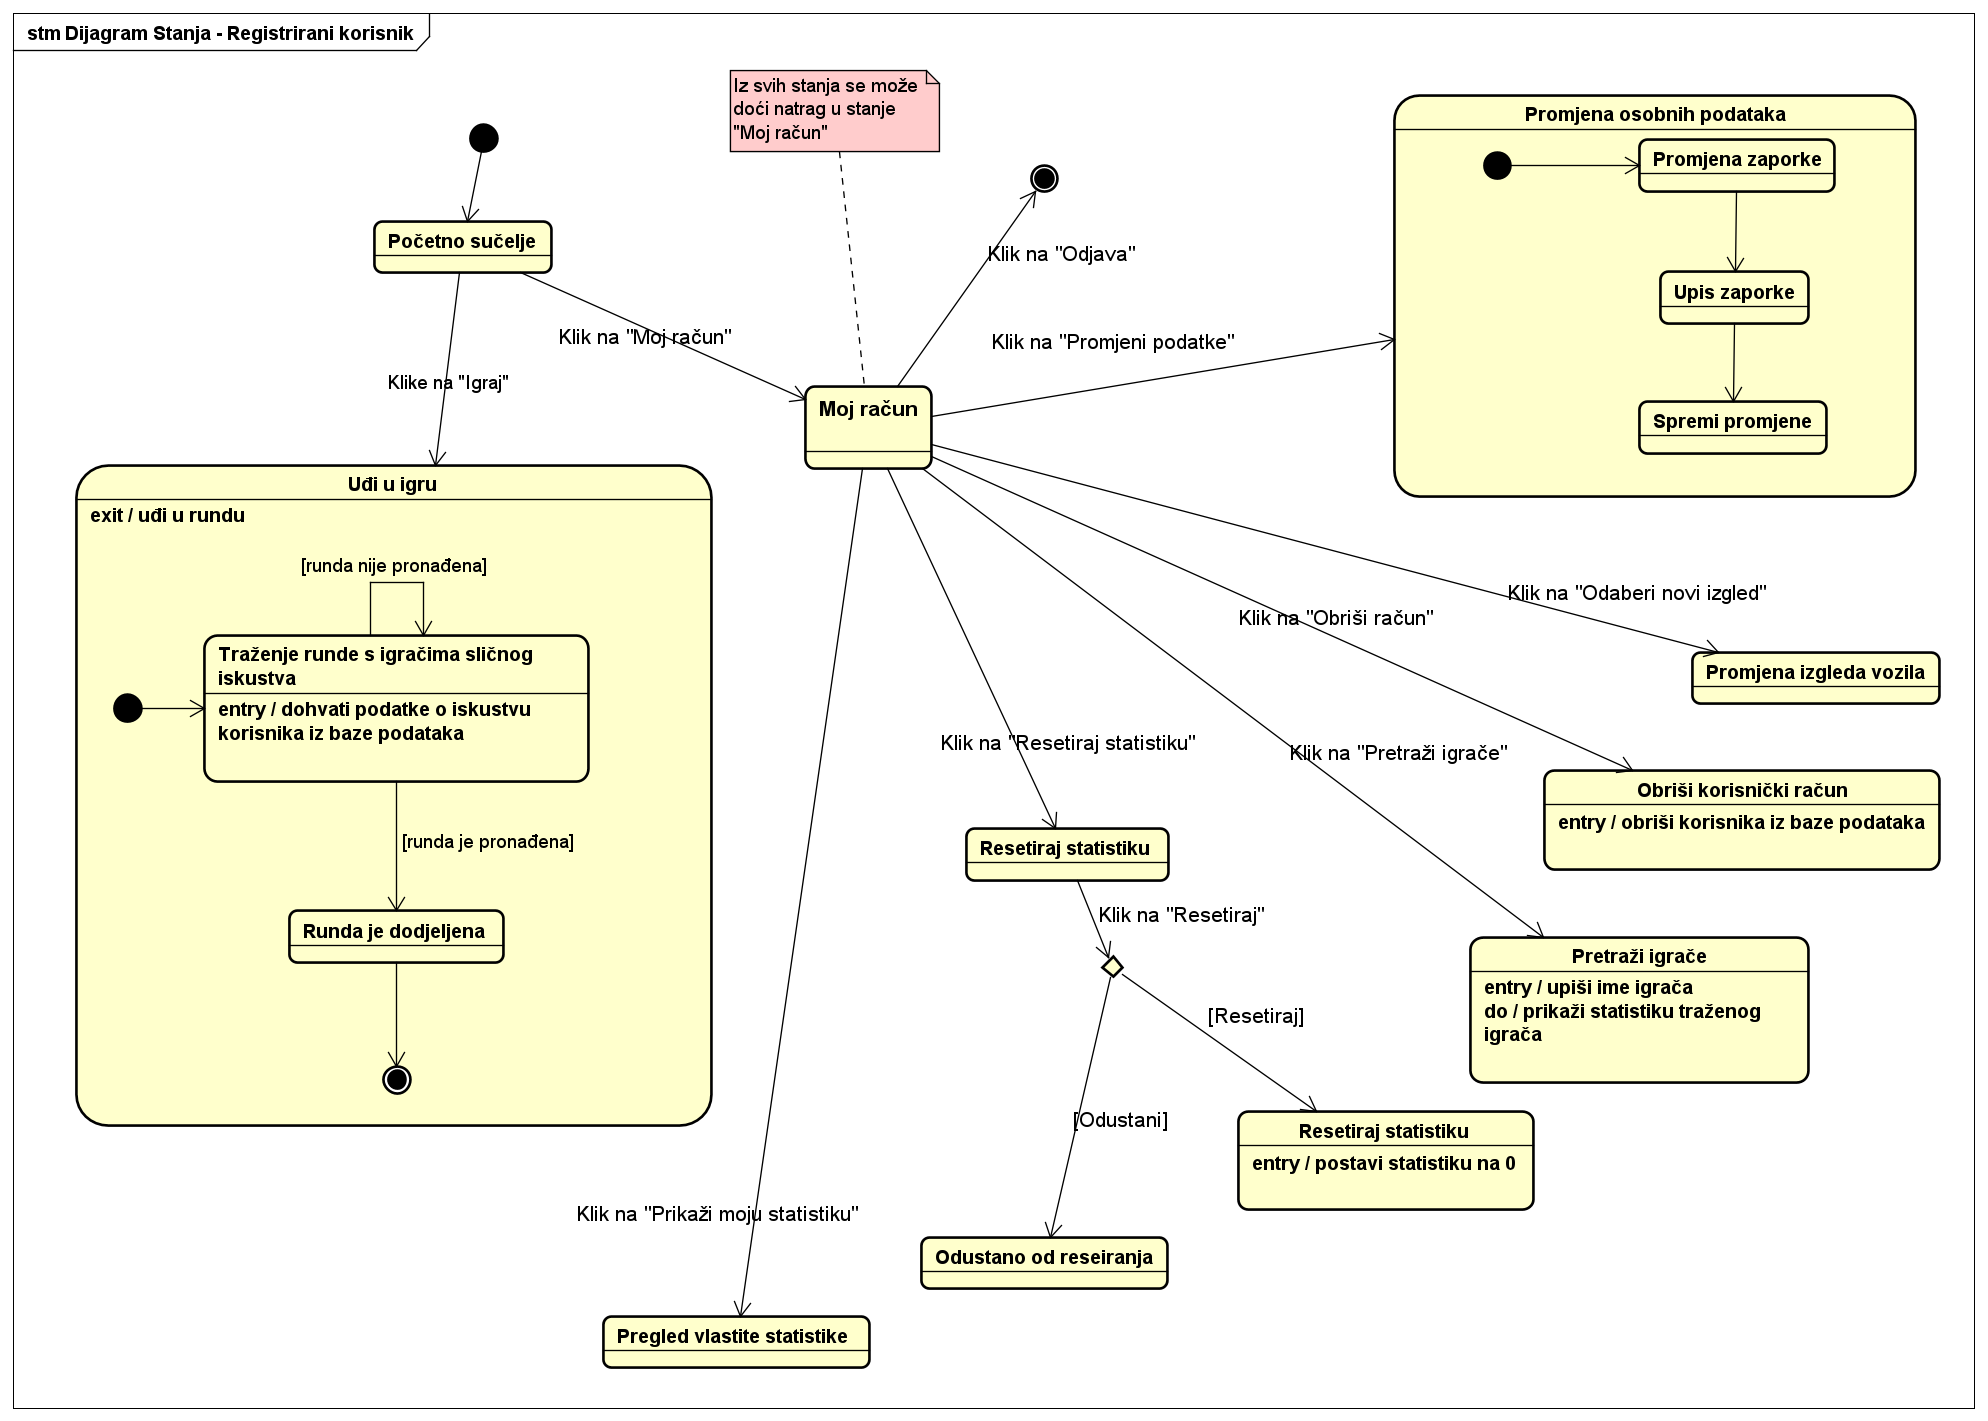
\includegraphics[width=17.5cm,height=12.5cm]{Dijagram Stanja - Registrirani korisnik}
				\caption{Dijagram stanja}
				\label{fig:stm}

			\end{figure}
			
			\eject 
			
	
		\section{Dijagram aktivnosti}
		
			{UML dijagram aktivnosti modelira ponašanja nizom aktivnosti, ali pritom se prijelaz iz jedne aktivnosti u drugu ne potiče nekim događajem. Priloženi dijagram aktivnosti prikazuje ulazak registriranog korisnika u igru. Korisnik se najprije prijavljuje u sustav sa svojim podacima. Akcije koje slijede su postupak prijave korisnika sve dok baza podataka ne vrati tražene podatke ili ih ne pronađe što znači da prijava nije uspjela. Nakon prijave, korisnik će ući u igru. Web preglednik će od servera tražiti dodjelu runde. Na serveru će se dogoditi dvije akcije. Prvo će iz baze podataka dohvatiti razinu iskustva tog korisnika, a zatim pronaći rundu s igračima slične razine iskustva. Ukoliko pronađe rundu, korisnik će uspješno ući u igru, a u suprotnom će se ponoviti traženje runde.}
			 
			\begin{figure}[h]
			 	\centering
			 	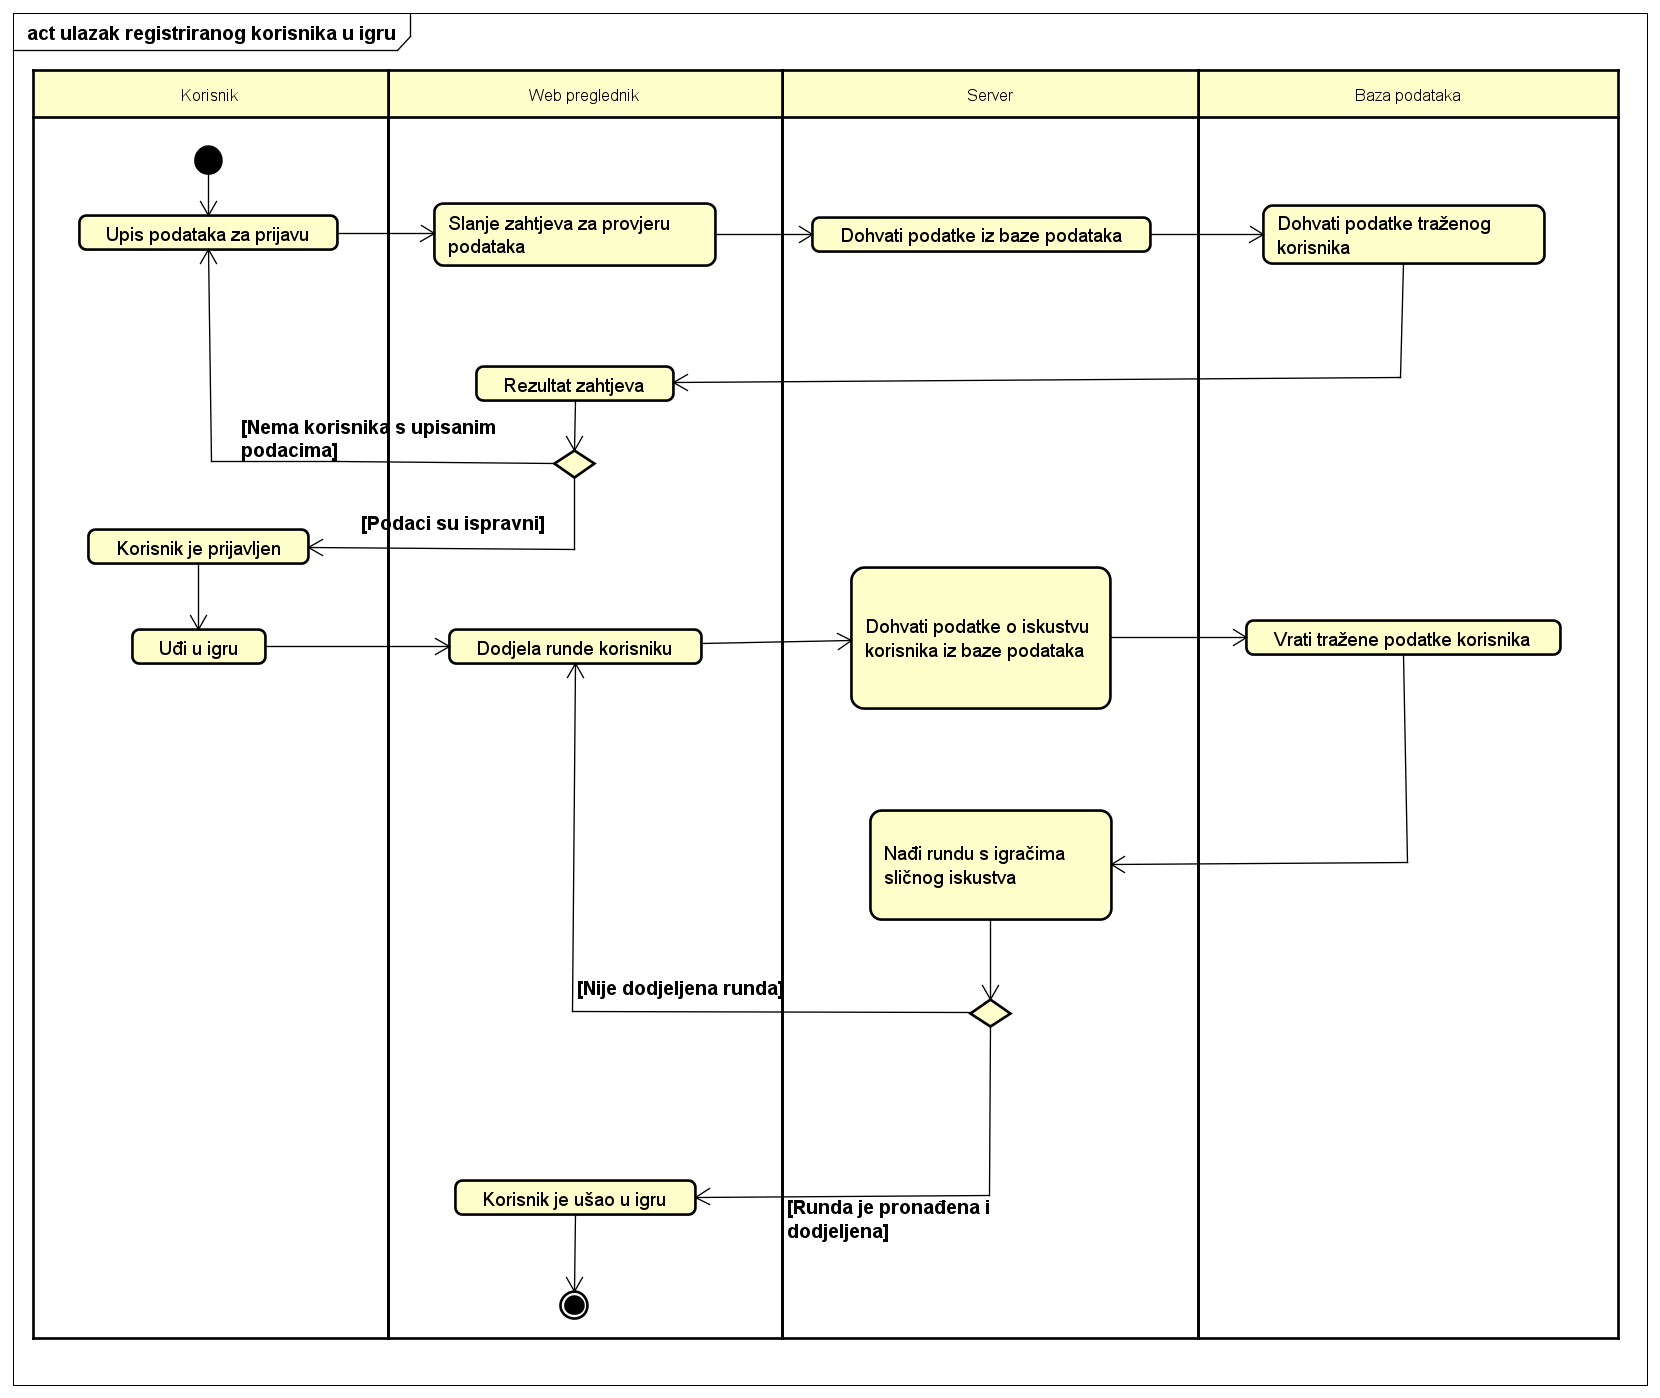
\includegraphics[width=17.5cm,height=12.5cm]{activityDiagram}
			 	\caption{Dijagram aktivnosti}
			 	\label{fig:act}
			\end{figure}
			
			\eject
		
		\newpage
		\section{Dijagram komponenti}
			
			 {Dijagram komponenti prikazuje specifikaciju arhitekture programske potpore. Vizualizira organizaciju i međuovisnosti između implementacijskih komponenata. }
			 
			 \begin{figure}[h]
			 	\centering
			 	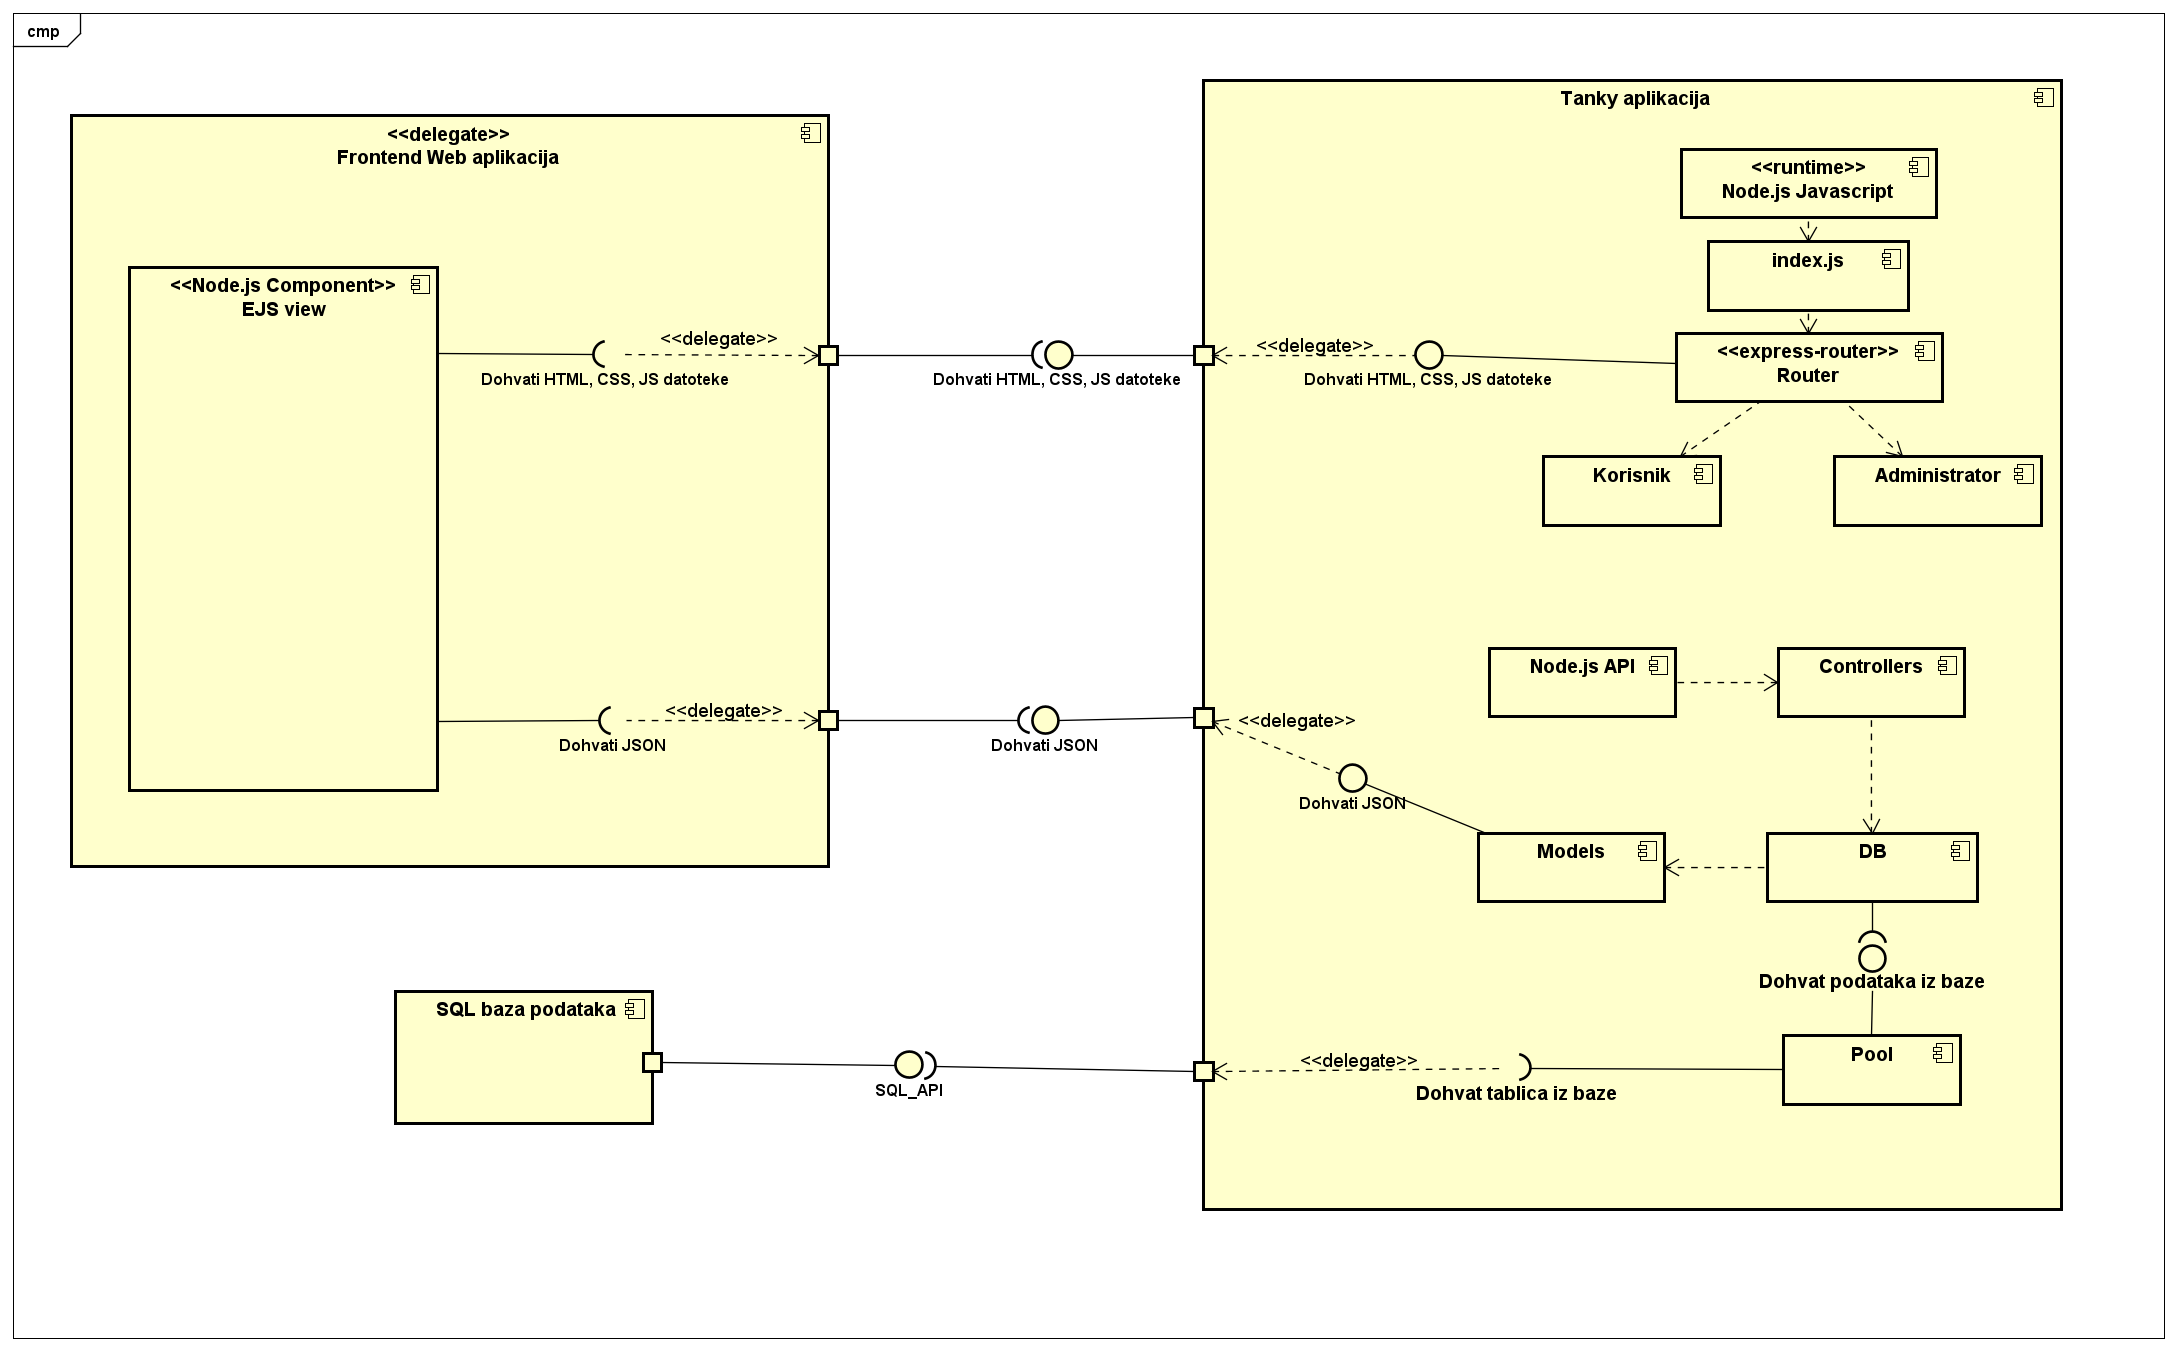
\includegraphics[width=17.5cm,height=12.5cm]{Component Diagram0}
			 	\caption{Dijagram komponenti}
			 	\label{fig:cmp}
			 \end{figure}